\documentclass[10pt,a4paper]{article}
\usepackage[a4paper,top=1.25cm,bottom=1.3cm,left=1.55cm,right=1.55cm]{geometry}
\usepackage{fontspec}
\setmainfont{Inter}[Scale=0.93]
\newfontfamily\rupeefont{DejaVu Sans}
\newcommand{\rs}{{\rupeefont ₹}}
\usepackage{xcolor,graphicx,tabularx,booktabs,enumitem,titlesec,array,amsmath}
\usepackage{tikz}
\usetikzlibrary{arrows.meta,positioning,fit,calc}
\usepackage[hidelinks]{hyperref}
\definecolor{ink}{HTML}{1B2130}
\definecolor{acc}{HTML}{2F62D6}
\definecolor{accsoft}{HTML}{E8EEFC}
\definecolor{gold}{HTML}{C99A1E}
\definecolor{muted}{HTML}{5A6273}
\color{ink}
\setlength{\parindent}{0pt}
\setlength{\parskip}{2.5pt}
\linespread{1.04}
\titleformat{\section}{\normalsize\bfseries\color{acc}}{\thesection.}{0.45em}{}
\titlespacing*{\section}{0pt}{6pt}{2.5pt}
\titleformat{\subsection}{\small\bfseries}{\thesubsection}{0.4em}{}
\titlespacing*{\subsection}{0pt}{4pt}{1.5pt}
\setlist{nosep,leftmargin=1.1em,itemsep=1.2pt}
\pagestyle{empty}
\begin{document}

% ---------- header ----------
\begin{minipage}[t]{0.70\textwidth}
{\LARGE\bfseries Learning Money by Living It}\\[1pt]
{\color{muted}A pixel-art life simulation that teaches financial literacy by letting students live it}
\end{minipage}\hfill
\begin{minipage}[t]{0.28\textwidth}\raggedleft
{\bfseries Team No.: 97}\\[1pt]
{\small\color{muted}M1 --- Approach}
\end{minipage}

\vspace{3pt}
{\color{acc}\rule{\textwidth}{1.2pt}}
\vspace{-2pt}

{\small\textbf{Problem statement:} Empowering the Next Generation Through Financial Literacy (Vanguard): design a digital experience that students want, for Grades 11--12 students from underserved communities across Hyderabad.}

\section{Problem Statement and Our Understanding}
\begin{itemize}
  \item \textbf{Audience and scale.} Intermediate (Grade 11--12) students from underserved communities in Hyderabad, starting with $\sim$1,500 students delivered through partner NGOs and designed to scale beyond that.
  \item \textbf{Scope.} Four pillars: \emph{plan \& budget} (needs vs.\ wants, choices, goals), \emph{save \& manage} (habits, spending, unexpected needs), \emph{understand investing} (risk, time, compounding, diversification), and \emph{stay financially safe} (protecting information, spotting suspicious offers).
  \item \textbf{What ``financial literacy'' means here.} Not finance as an academic subject, but the knowledge, habits and confidence to make sensible decisions with one's \emph{own} money: pocket money, a scholarship, UPI payments, a first salary.
  \item \textbf{What makes it hard.} (i) Relatability: concepts must map onto decisions these students actually face, without jargon. (ii) Learning must be demonstrable, not just engagement. (iii) Delivery happens through NGOs, on shared low-end phones, in several languages. (iv) The users are minors, so privacy matters. (v) Guardrail: \emph{educate, do not recommend investments; simulations are assumptions, not promises.}
\end{itemize}

\section{Idea / Abstract}
\colorbox{accsoft}{\parbox{\dimexpr\textwidth-2\fboxsep}{\small
Our solution is a browser-based, pixel-art role-playing game. A student creates an avatar, answers a short onboarding quiz, and lives a compressed life in three stages: \textbf{Intermediate student $\rightarrow$ first salary $\rightarrow$ earning more}. Each stage is a series of \textbf{tasks presented as ``money battles''}: a scam call, a festival budget, a medical emergency. The student chooses what to do, and the game shows the consequence, sometimes much later.
\textbf{The game is designed to teach the concepts while being relatable to the target demographic}: every task is set in familiar Hyderabad situations, framed for the student's own background, and priced relative to their own pocket money.
\textbf{The teaching itself is done through short abstract animations}: shapes and on-screen text that explain the concept behind each decision. They play right after the choice and can be replayed later.
Mistakes are recorded and return in new forms until learned. The game ends with an epilogue at age $\sim$55--60 showing where the student's choices led, and a progress report emailed to their NGO facilitator.}}

\section{High-Level Approach}
\subsection{Player journey (pipeline)}
\vspace{1pt}
\begin{center}
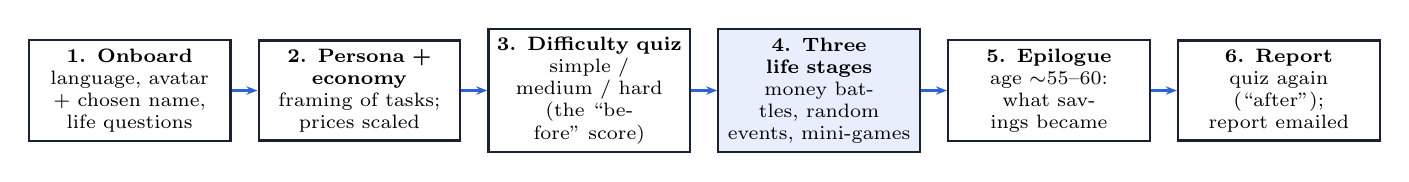
\begin{tikzpicture}[
  box/.style={draw=ink,line width=0.8pt,fill=white,align=center,text width=2.35cm,minimum height=1.25cm,font=\scriptsize,inner sep=3pt},
  hi/.style={box,fill=accsoft},
  arr/.style={-{Stealth[length=4pt]},line width=0.8pt,color=acc}]
\node[box] (a) {\textbf{1. Onboard}\\language, avatar\\+ chosen name,\\life questions};
\node[box,right=0.33cm of a] (b) {\textbf{2. Persona +}\\\textbf{economy}\\framing of tasks;\\prices scaled};
\node[box,right=0.33cm of b] (c) {\textbf{3. Difficulty quiz}\\simple / medium / hard\\(the ``before'' score)};
\node[hi,right=0.33cm of c] (d) {\textbf{4. Three life stages}\\money battles, random\\events, mini-games};
\node[box,right=0.33cm of d] (e) {\textbf{5. Epilogue}\\age $\sim$55--60:\\what savings became};
\node[box,right=0.33cm of e] (f) {\textbf{6. Report}\\quiz again (``after'');\\report emailed};
\foreach \x/\y in {a/b,b/c,c/d,d/e,e/f}{\draw[arr] (\x) -- (\y);}
\end{tikzpicture}
\end{center}
\vspace{-3pt}

\subsection{Core teaching loop and the ``money battle'' screen}
\begin{minipage}[t]{0.47\textwidth}
\vspace{0pt}
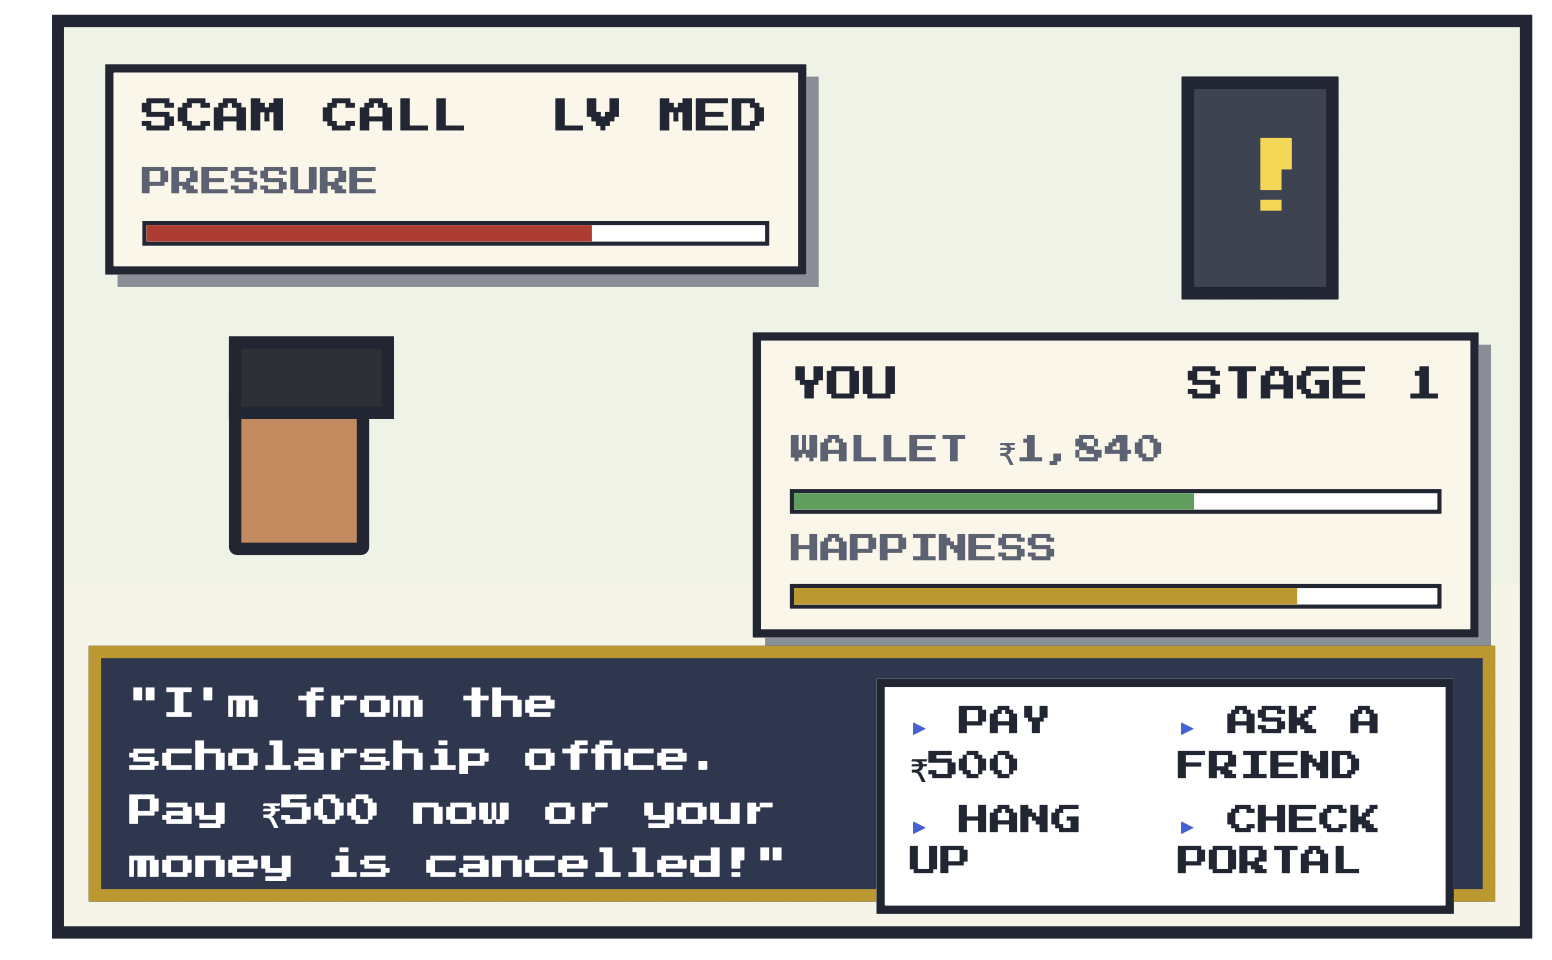
\includegraphics[width=\linewidth]{battle.png}\\[-1pt]
{\scriptsize\color{muted}Concept mock-up (original art). The opponent is the situation and its bar is the pressure it puts on the player. The player's bars are \emph{wallet} and \emph{happiness}. Each turn offers 2--4 choices.}
\end{minipage}\hfill
\begin{minipage}[t]{0.505\textwidth}
\vspace{0pt}
\small
\begin{enumerate}[leftmargin=1.2em]
  \item \textbf{Situation:} a task from the student's difficulty bucket, framed for their persona.
  \item \textbf{Choice:} 2--4 options with pictures (and audio).
  \item \textbf{Consequence:} the status bars change at once. Some choices also schedule later effects (an EMI deducted every month; money lent that never comes back).
  \item \textbf{Teach:} a 10--20\,s abstract animation explains the concept behind the decision. It is added to a \textbf{replay library}.
  \item \textbf{Remember:} a weak choice puts its concept in a \textbf{mistake bank}. The concept returns later in a new disguise and is cleared only when answered correctly.
\end{enumerate}
\textbf{Happiness bar.} It mirrors the student's real mental state, including the gap between feeling good now and paying for it later. An impulsive treat, such as ordering a \rs500 meal online instead of a \rs20 snack, \emph{raises} happiness at once. The next day, if friends invite the student to a paid turf cricket match they can no longer afford, they are forced to say no and happiness \emph{drops}. It also drops when low funds lock them out of mini-games, or when they get scammed (\emph{Pay \rs500} above drains wallet and happiness together). At zero the task restarts. The lesson is felt, not told: impulse buys feel good for a day and cost you the things you actually wanted.
\end{minipage}

\vspace{3pt}
\subsection{Key design decisions}
{\small
\begin{tabularx}{\textwidth}{@{}>{\bfseries}p{2.6cm}X@{}}
\toprule
Persona & Assigned from life questions, including an indirect pocket-money range; shown to the student, who can switch. It changes only the \emph{framing and analogies} of each task (e.g.\ the same scam arrives as an ``OTP sent by mistake'' on a parent's phone, or as a fake scholarship officer), never its difficulty.\\
Difficulty & A 5-question onboarding quiz places the student in a \emph{simple / medium / hard} bucket. Tasks are drawn from buckets organised by pillar $\times$ difficulty.\\
Economy scaling & Everyone starts with the same in-game amount $S$. Prices are scaled so that each item costs the same share of money as in the student's real life: in-game price $=$ real price $\times\, S \,/\,$ monthly pocket money.\\
Consequences & A weak choice leads to a detour of consequence tasks, then the path rejoins. A critical failure (falling for a scam, going broke, happiness at zero) restarts the task.\\
Mini-games & Appear at random and can be skipped. They give an in-game reward, but are locked while any status bar is below its threshold.\\
Info \& replay & An always-available info button shows the current status (bars, savings, active commitments, open mistakes). The replay library re-plays past explainer animations.\\
End of game & An in-game ``what if'' screen replays the student's \emph{biggest mistake} with the choice they didn't make, using their own decision log. Separately, a \emph{progress report} (scores, before/after quiz, pillar progress) is emailed to the NGO facilitator with the guardian in CC. The ``what if'' is not part of the email.\\
Guardrail & Fictional assets only, never real products or tickers. Every projection is labelled ``assumes $X$\% a year; real returns vary and can be negative''.\\
\bottomrule
\end{tabularx}}

\section{Proposed Architecture}
\vspace{-2pt}
\begin{center}
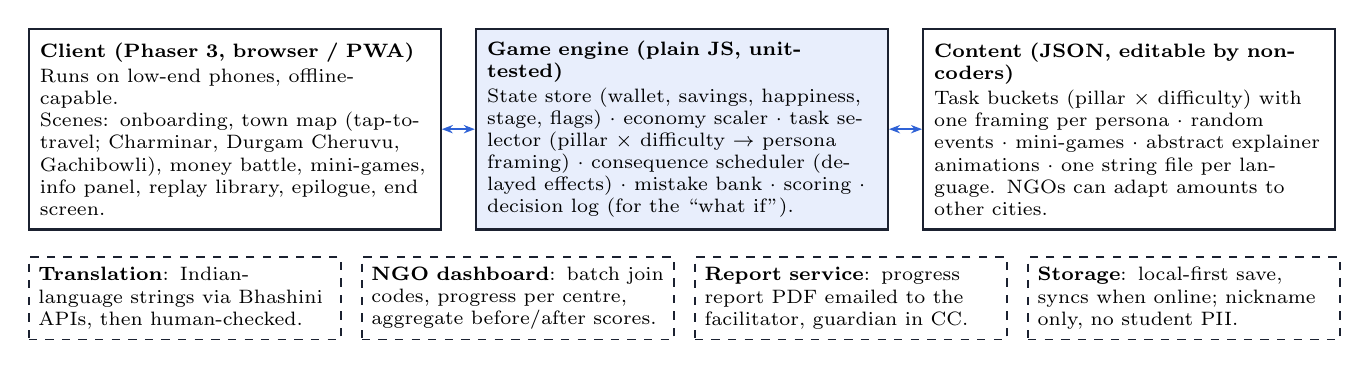
\begin{tikzpicture}[
  lay/.style={draw=ink,line width=0.8pt,align=left,text width=4.95cm,font=\scriptsize,inner sep=4pt,minimum height=2.55cm},
  svc/.style={draw=ink,dashed,line width=0.7pt,align=left,text width=3.72cm,font=\scriptsize,inner sep=3.5pt,minimum height=1.05cm},
  arr/.style={{Stealth[length=4pt]}-{Stealth[length=4pt]},line width=0.8pt,color=acc}]
\node[lay] (cl) {\textbf{Client (Phaser 3, browser / PWA)}\\[1pt]
Runs on low-end phones, offline-capable.\\Scenes: onboarding, town map (tap-to-travel; Charminar, Durgam Cheruvu, Gachibowli), money battle, mini-games, info panel, replay library, epilogue, end screen.};
\node[lay,fill=accsoft,right=0.42cm of cl] (en) {\textbf{Game engine (plain JS, unit-tested)}\\[1pt]
State store (wallet, savings, happiness, stage, flags) $\cdot$ economy scaler $\cdot$ task selector (pillar $\times$ difficulty $\rightarrow$ persona framing) $\cdot$ consequence scheduler (delayed effects) $\cdot$ mistake bank $\cdot$ scoring $\cdot$ decision log (for the ``what if'').};
\node[lay,right=0.42cm of en] (ct) {\textbf{Content (JSON, editable by non-coders)}\\[1pt]
Task buckets (pillar $\times$ difficulty) with one framing per persona $\cdot$ random events $\cdot$ mini-games $\cdot$ abstract explainer animations $\cdot$ one string file per language. NGOs can adapt amounts to other cities.};
\draw[arr] (cl) -- (en); \draw[arr] (en) -- (ct);
\node[svc,below=0.32cm of cl.south west,anchor=north west] (s1) {\textbf{Translation}: Indian-language strings via Bhashini APIs, then human-checked.};
\node[svc,right=0.24cm of s1] (s2) {\textbf{NGO dashboard}: batch join codes, progress per centre, aggregate before/after scores.};
\node[svc,right=0.24cm of s2] (s3) {\textbf{Report service}: progress report PDF emailed to the facilitator, guardian in CC.};
\node[svc,right=0.24cm of s3] (s4) {\textbf{Storage}: local-first save, syncs when online; nickname only, no student PII.};
\end{tikzpicture}
\end{center}
\vspace{-4pt}

\section{Planned Testing Methodology}
{\small
\begin{tabularx}{\textwidth}{@{}>{\bfseries}p{3.0cm}X@{}}
\toprule
Learning gain & \textbf{Before/after quiz:} the 5-question onboarding difficulty quiz (time value of money, interest on a loan, compound interest, inflation, diversification) is asked again after the epilogue. The score difference is the learning gain, reported per student and per pillar, and aggregated per NGO batch. In-game choices are also scored on NCFE's framework (knowledge $\geq$6/8, behaviour $\geq$6/9, attitude $\geq$3/5), with the 2019 national adult figure of 27\% as a reference point.\\
Usability & Unguided play tests (peers as proxies during the hackathon; target-age students in an NGO pilot): time to finish the first task without help, number of help requests, and drop-off points.\\
Engine correctness & Unit tests for the economy scaler, consequence scheduler, mistake bank, scoring and ``what if'' replay, run on seeded game histories. Schema validation that every task has a difficulty tag, all persona framings and valid effects.\\
Devices \& network & Chrome DevTools throttling (slow 3G, 4$\times$ CPU slowdown) on a budget-Android profile; a full offline play-through; target load time under 5\,s.\\
Language & An automated check that every string key exists in each language file, plus a screenshot review per language.\\
Report \& privacy & Reports generated from seeded histories and sent to sandbox inboxes to verify the recipients and content. A content checklist (no product recommendations; every projection labelled as an assumption) and no personal data stored beyond a nickname.\\
\bottomrule
\end{tabularx}}

\end{document}
